\documentclass[a4paper]{article}

\usepackage[utf8]{inputenc}
\usepackage[top=1.5cm, bottom=1.5cm, left=1.5cm, right=1.5cm]{geometry}
\usepackage[pdftex]{graphicx}
\usepackage{color}
\usepackage{makeidx}

\newcommand{\HRule}{\rule{\linewidth}{0.5mm}}
\makeindex
\begin{document}

\begin{titlepage}



\begin{center}

{\vspace*{8.5cm}}

% Upper part of the page


\textsc{\LARGE University of Aberystwyth}\\[1.5cm]

\textsc{\Large First year group project}\\[0.5cm]


% Title
\HRule \\[0.4cm]
{ \huge \bfseries UML2 Java}\\[0.4cm]

\HRule \\[1.5cm]

% Author and supervisor
\begin{minipage}{0.4\textwidth}
\begin{center} \large
\emph{Authors:}\\
Daniel Mal\'{y},\\ Samuel Sherar,\\ Lee Smith
\end{center}
\end{minipage}

\vfill


\end{center}

\end{titlepage}


\begin{center}\LARGE{UML2Java Graphical Designer}
\end{center}

\texttt{UML2Java} is a Graphic User Interface program that allows a user to create UML2 class diagrams. The program will then output the class files from the created class diagram including all relevant fields, methods and relationships to other classes. The UML designer was created as a requirement for our first year group project. 

\newpage
\tableofcontents 
\newpage

\section{File Menu} 

\subsection{Create new Class Diagram} \index{File!Create new diagram}
To create a new Class Diagram, go to the top menu bar and press \texttt{File $\rightarrow$ New}

\begin{center} 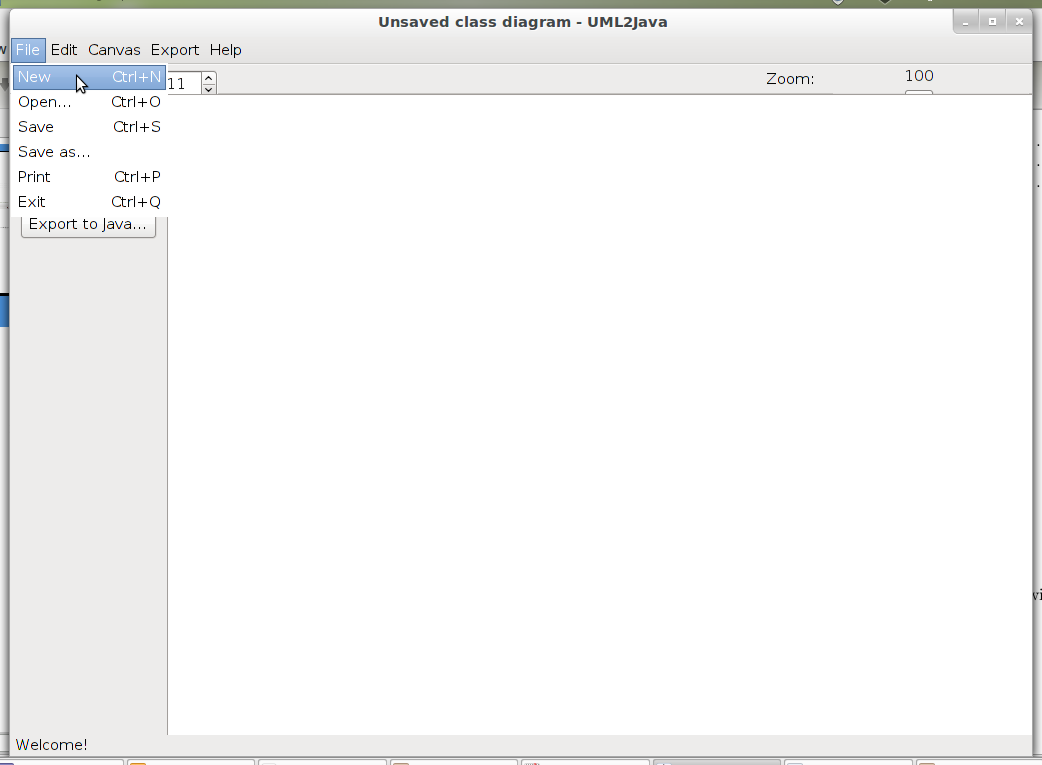
\includegraphics[trim = 0pt 500pt 0pt 0pt, clip, scale=0.4]{./images/file-new.png} \end{center}

\subsection{Open an existing diagram} \index{File!Open existing diagram}
To open a previously saved diagram, go to the top menu bar and press \texttt{File $\rightarrow$ Open...} or simply press \texttt{CTRL+O}
This will open up a new window asking for the location of the file you wish to open
\begin{center} 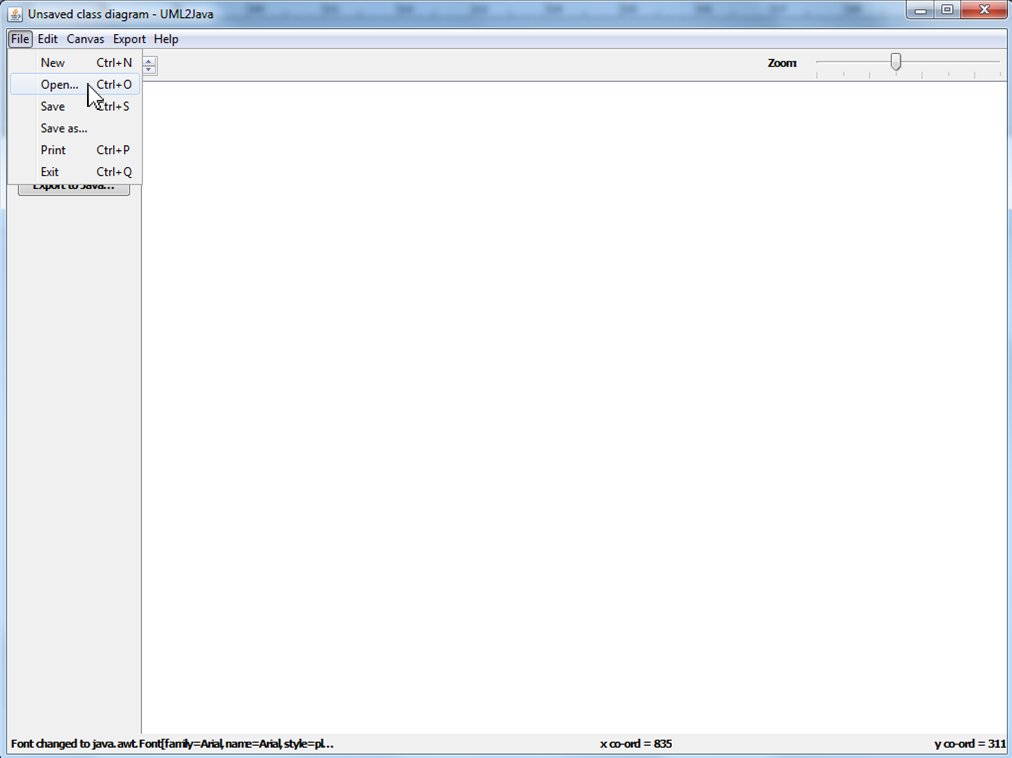
\includegraphics[trim = 0pt 300pt 700pt 0pt, clip, scale=0.4]{./images/file-open1.png}     
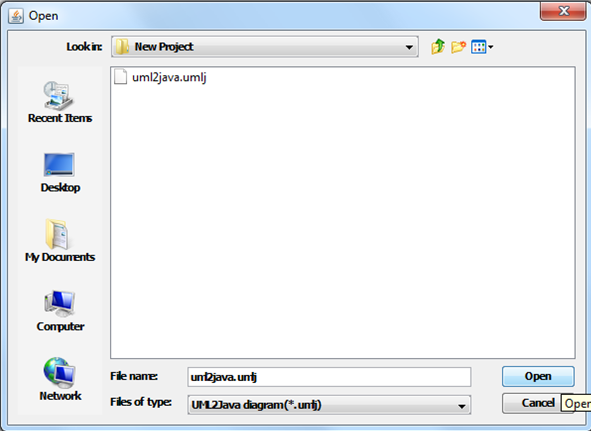
\includegraphics[scale=0.4]{./images/file-open2.png} \end{center}

\subsection{Saving a diagram} \index{File!Save a Diagram}
To save a diagram, go to the top menu bar and press \texttt{File $\rightarrow$ Save/Save as...} or simply press \texttt{CTRL+S}
\begin{center} 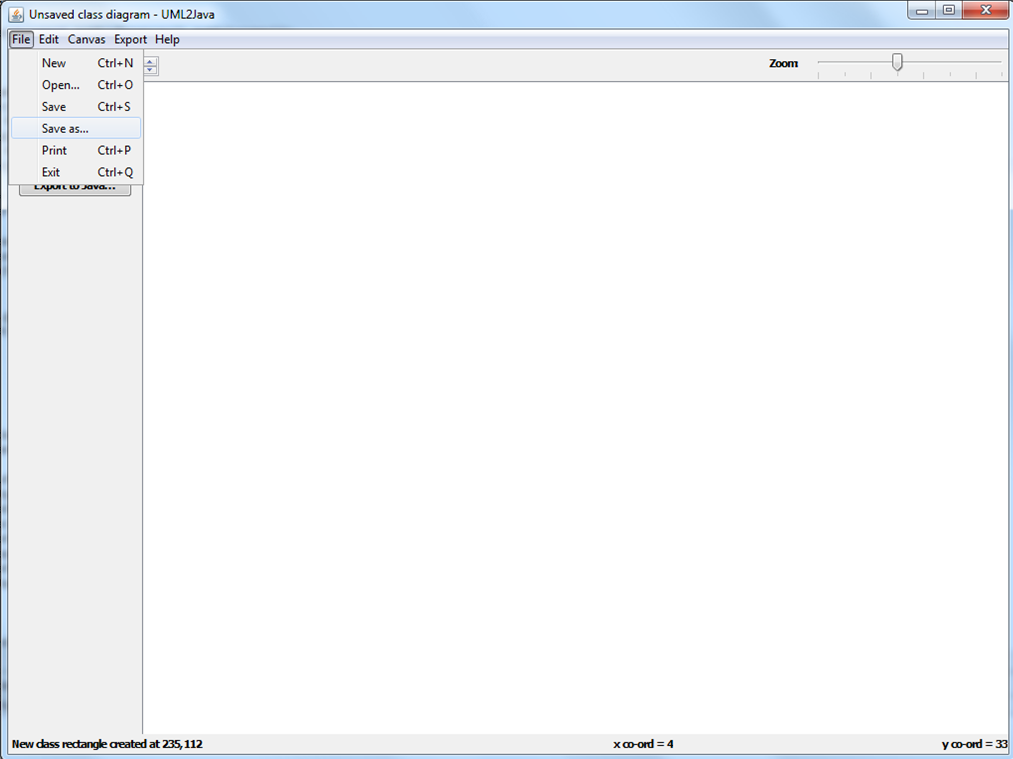
\includegraphics[trim = 0pt 300pt 700pt 0pt, clip, scale=0.4]{./images/file-save1.png}     
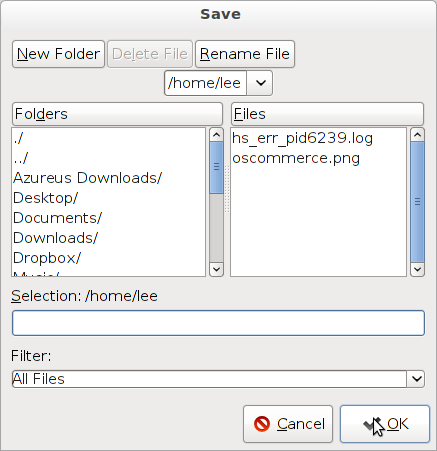
\includegraphics[scale=0.4]{./images/file-save2.png} \end{center}
\newpage

\subsection{Printing a Diagram} \index{File!Printing a diagram}
To print a created diagram, go to the top bar and press \texttt{File $\rightarrow$ Print} or simply press \texttt{CTRL+P} and select the desired printer from the open window

\subsection{Exiting the Designer} \index{File!Exiting UML2Java}
To end the current session in \texttt{UML2Java}

\section{Edit Menu}
\subsection{Undoing an Action} \index{Edit!Undo}
If you require to undo the previous action, go to the top bar and press \texttt{Edit $\rightarrow$ Undo} or press \texttt{CTRL+Z} from the keyboard
\begin{center} 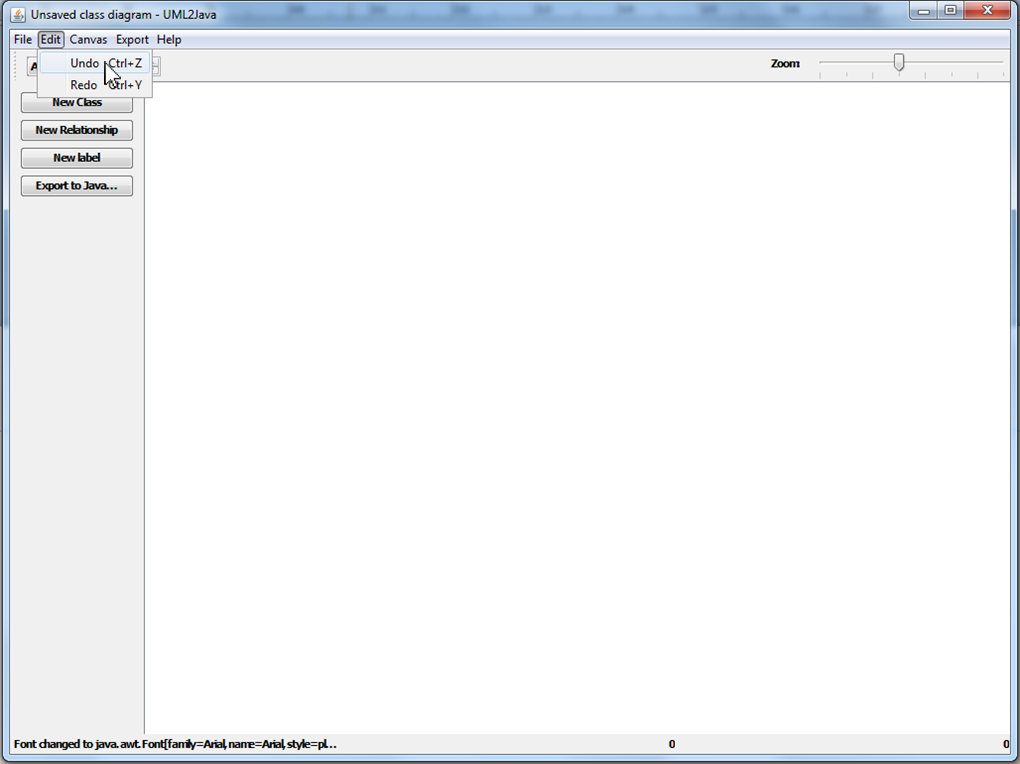
\includegraphics[trim = 0pt 500pt 0pt 0pt, clip, scale=0.45]{./images/edit-undo.png} \end{center}
\subsection{Redoing an Action} \index{Edit!Redo}
if you need to redo a previously undone action, simply go to the top bar and press \texttt{Edit $\rightarrow$ Redo} or press \texttt{CTRL+Y} from your keyboard
\begin{center} 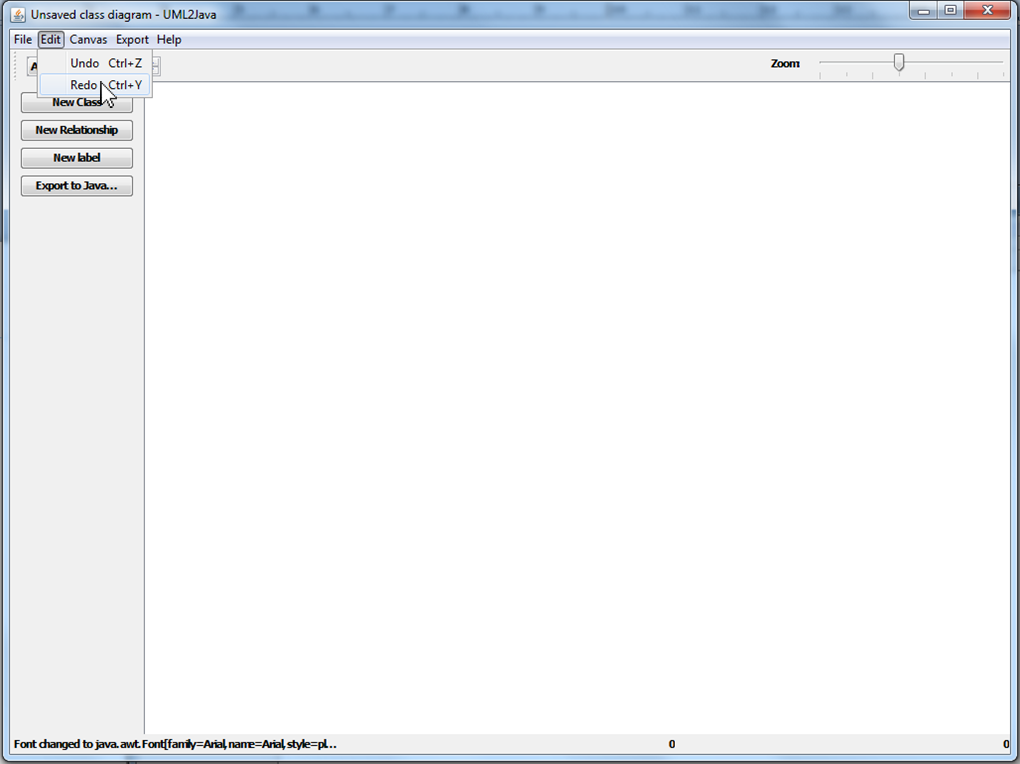
\includegraphics[trim = 0pt 500pt 0pt 0pt, clip, scale=0.45]{./images/edit-redo.png} \end{center}

\section{Editing Canvas Settings}
\subsection{Resize the Canvas} \index{Canvas Settings!Resize}
If you require a different canvas size , you can do this from the top menu, pressing \texttt{Canvas $\rightarrow$ Resize}
\newpage %can be deleted once images become available

\subsection{Fitting to Diagram} \index{Canvas Settings!Fit to Diagram}
The canvas menu option also allows you to resize the canvas to a state where all of the current contents of the diagram will be able to be seen with little white space around the resulting design, to achieve this press \texttt{Canvas $\rightarrow$ Fit to Diagram}
\begin{center} \includegraphics[trim = 0pt 500pt 0pt 0pt, clip, scale=0.45]{./images/canvas-fitto.png} \end{center}

\section{Exporting}
\subsection{Export to Code} \index{Exporting!Code}
To create the code files of your created diagram, go to the top bar and select \texttt{Export $\rightarrow$ Code} this will generate the .java files of your created diagram, it will take into account any relationships you have created between classes, any variable declarations you have made, and methods you have created. Or you can go to the left menu bar and select \texttt{Export to Java} from the list there. \par

\begin{center}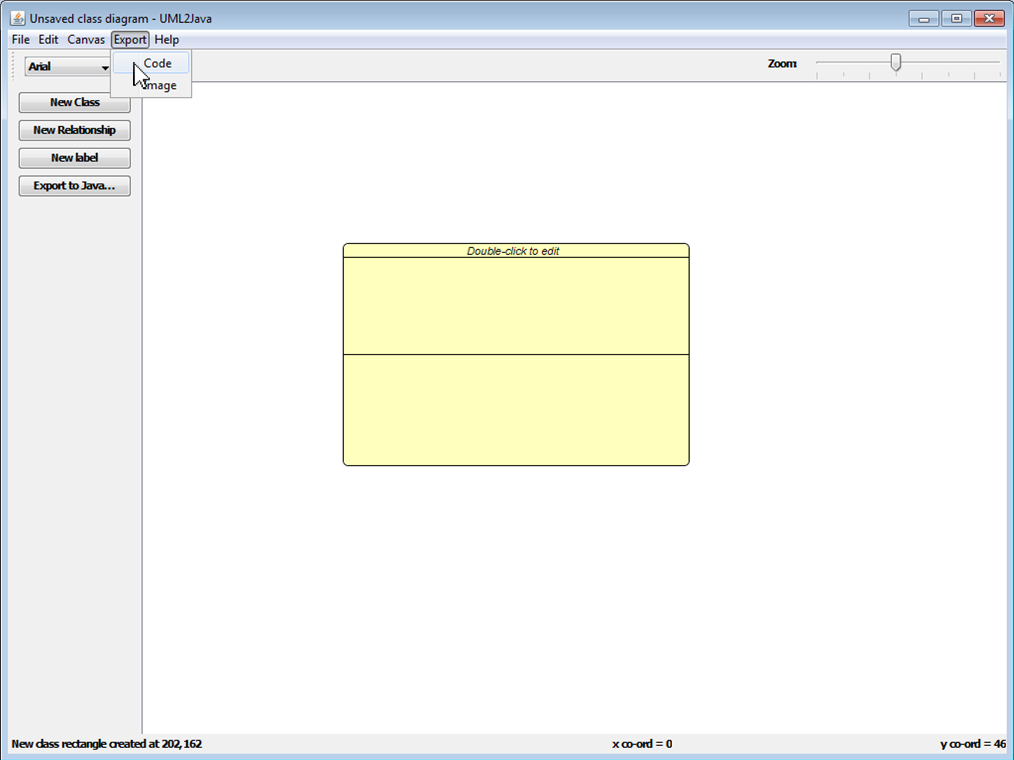
\includegraphics[trim = 0pt 300pt 700pt 0pt, clip, scale=0.4]{./images/export-code1.png}
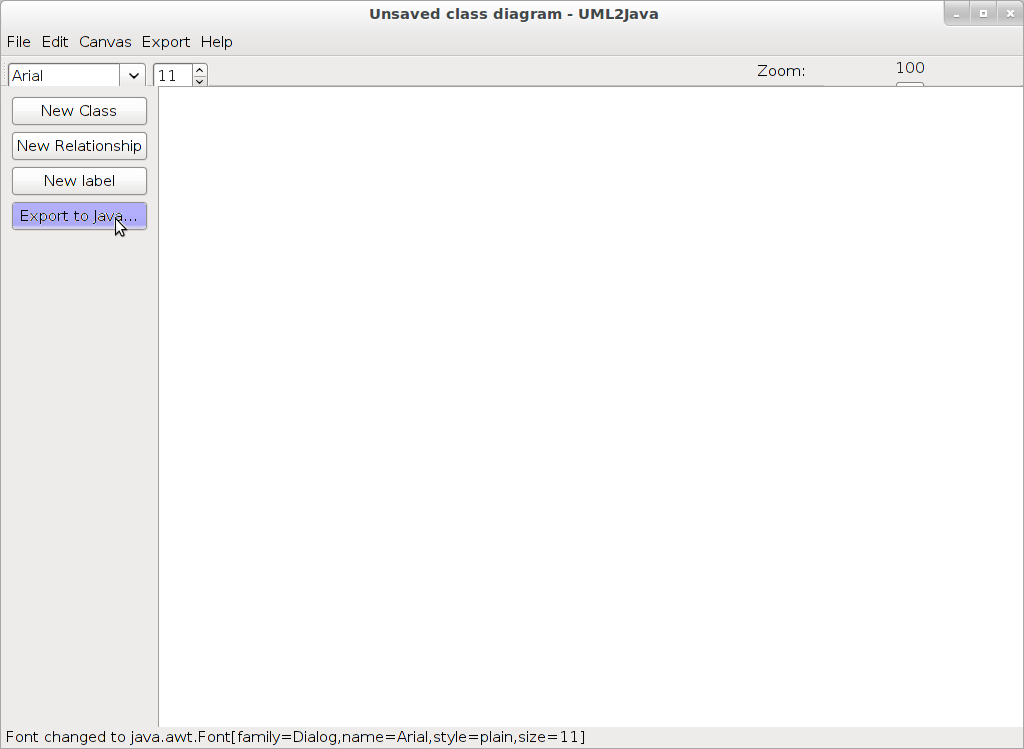
\includegraphics[trim = 0pt 300pt 700pt 0pt, clip, scale=0.4]{./images/export-code2.png} \end{center}

\subsection{Export Image of Diagram}\index{Exporting!Image}
To create an image file of the class diagram you have created, go to \texttt{Export $\rightarrow$ Image} and an save box will appear, where you can select the location of where you wish to save the file and also the file type, either \texttt{.png} or \texttt{.jpg}

\newpage
\section{Adding Elements to the Class Diagram}
\subsection{Adding a new class}\index{Adding to diagram!Add new Class}
To create a new class on the diagram, go to the left-hand menu and select \texttt{New Class}
\begin{center}\includegraphics[trim = 0pt 300pt 700pt 0pt, clip, scale=0.4]{./images/addnewclass1.png} \end{center}
To make sure that you have selected to add a new class, once pressed a message will appear in the status bar at the bottom of the window
\begin{center}\includegraphics[trim = 0pt 0pt 500pt 675pt, clip, scale=0.7]{./images/addnewclass2.png} \end{center}
To add the class to the diagram, left-click on the white canvas and your new class will appear
\begin{center}\includegraphics[scale=0.3]{./images/addnewclass3.png} \end{center}
You will recieve confirmation via the status bar at the bottom of the screen, giving the x and y co-ordinates of the generated class box
\begin{center}\includegraphics[trim = 0pt 0pt 500pt 675pt , clip, scale=0.7]{./images/addnewclass3.png} \end{center}
\newpage
\subsection{Adding a new Relationship between classes}\index{Adding to diagram!Add new Relationship}
To add a relationship between two classes, press \texttt{New Relationship} from the left-hand menu




\newpage
\printindex
\end{document}
